\subsection{Exercise~1.3}
\label{exercise 1.3}



\subsubsection{Verifying that the Zariski Topology is a Topology}

Let~$R$ be a commutative ring and let~$X ≔ \spec R$.

For~$E = ∅$ we have~$V E = X$, and for $E = R$ we have~$V E = ∅$.
We have for every family~$(E_α)_{α ∈ A}$ of subsets of~$R$ the equality
\[
	⋂_{α ∈ A} V E_α
	=
	V ⋃_{α ∈ A} E_α \,.
\]
This shows that intersections of closed sets are again closed.
To show that finite unions of closed sets are again closed we use the following observation:

\begin{lemma}
	\label{product in prime ideal}
	Let~$R$ be a commutative ring and let~$𝔭$ be a prime ideal of~$R$.
	Let~$E$ and~$F$ be two subsets of~$R$.
	Then~$E F ⊆ 𝔭$ if and only if~$E ⊆ 𝔭$ or~$F ⊆ 𝔭$.
\end{lemma}

\begin{proof}
	If~$E ⊆ 𝔭$ or~$F ⊆ 𝔭$ then also~$EF ⊆ 𝔭$ because~$𝔭$ is in an ideal.
	Suppose conversely that neither~$E ⊆ 𝔭$ nor~$F ⊆ 𝔭$.
	Then there exist elements~$x ∈ E$ and~$y ∈ F$ with~$x, y ∉ 𝔭$.
	It follows that also~$xy ∉ 𝔭$ because the ideal~$𝔭$ is prime.
	Consequently,~$EF ⊈ 𝔭$.
\end{proof}

It follows from the above \lcnamecref{product in prime ideal} that for all subsets~$E_1, \dotsc, E_n$ of~$R$, we have
\[
	V E_1 ∪ \dotsb ∪ V E_n
	=
	V (E_1 \dotsm E_n) \,.
\]
This shows that finite unions of closed subsets are again closed.



\subsubsection{The Spectrum of a Principal Ideal Domain}

Let~$R$ be a principal ideal domain.
This entails that~$R$ is a unique factorization domain.

The prime ideals of~$R$ are precisely the ideals of the form~$\genideal{p}$ with~$p$ irreducible in~$R$, together with the zero ideal.
Every nonzero prime ideal of~$R$ is already a maximal ideal.

\begin{lemma}
	Let~$R$ be a commutative ring and let~$E$ be a subset of~$R$.
	Then
	\[
		V E = V \genideal{E} \,.
	\]
\end{lemma}

\begin{proof}
	For every ideal~$I$ of~$R$ we have~$E ⊆ I$ if and only if~$\genideal{E} ⊆ I$.
	This holds in particular for prime ideals.
\end{proof}

\begin{corollary}
	Let~$R$ be a commutative ring.
	Every closed subset of~$R$ is of the form~$V I$ for some ideal~$I$ of~$R$.
	\qed
\end{corollary}

Let~$\genideal{p}$ be a prime ideal of~$R$, with~$p$ either irreducible or zero, and let~$I$ be any ideal of~$R$.
The ideal~$I$ is of the form~$I = \genideal{x}$ for some~$x ∈ R$.
We have~$I ⊆ \genideal{p}$ if and only if~$p$ divides~$x$.

If~$I$ is the zero ideal, then~$V I = \spec R$.
If the ideal~$I$ is nonzero, then its generator~$x$ is nonzero, and thus admits a prime decomposition~$x = p_1^{ν_1} \dotsm p_r^{ν_r}$, where~$p_1, \dotsc, p_r$ are pairwise non-equivalent irreducible elements of~$R$.
We then find that~$V I = \{ \genideal{p_1}, \dotsc, \genideal{p_r} \}$.

The closed subsets of~$X = \spec R$ are thus~$∅$ and~$X$, as well as all finite subsets not containing the point~$\genideal{0}$.
In other words, the subspace topology on~$X ∖ \{\genideal{0}\}$ is the cofinite topology, and the point~$\genideal{0}$ is dense in~$X$.



\subsubsection{The spectrum of~$ℤ$}

We can draw a picture of~$\spec ℤ$ as follows:
\begin{center}
	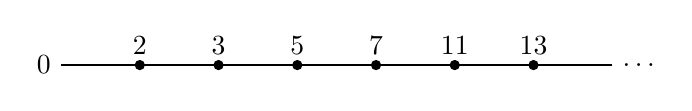
\begin{tikzpicture}[every path/.style={fill, thick}]
		\draw (0, 0) circle (0.05) node[above] {$\genideal{2}$};
		\draw (1, 0) circle (0.05) node[above] {$\genideal{3}$};
		\draw (2, 0) circle (0.05) node[above] {$\genideal{5}$};
		\draw (3, 0) circle (0.05) node[above] {$\genideal{7}$};
		\draw (4, 0) circle (0.05) node[above] {$\genideal{11}$};
		\draw (5, 0) circle (0.05) node[above] {$\genideal{13}$};
		\draw (-1, 0) node[left]{$\genideal{0}$} -- (6, 0) node[right]{$\dots$};
	\end{tikzpicture}
\end{center}
The elements~$\genideal{2}, \genideal{3}, \dotsc$ are drawn as points;
the topology on~$\{ \genideal{2}, \genideal{3}, \genideal{5}, \dotsc \}$ is the cofinite one.
The special element~$\genideal{0}$ of~$\spec ℤ$ is drawn as a line on which all other points lie.
In this way, every closed subspace of~$\spec ℤ$ that contains~$\genideal{0}$ must contain the line, and therefore also all points on it.



\subsubsection{The spectrum of~$ℂ[x]$}

The prime ideals in~$ℂ[x]$ are the ideals~$\genideal{x - λ}$ for~$λ ∈ ℂ$ together with the zero ideal, because the field~$ℂ$ is algebraically closed.
We may therefore draw~$\spec ℂ[x]$ as the complex plane, with the point~$λ ∈ ℂ$ representing the ideal~$\genideal{x - λ}$ and the entire plane representing the ideal~$\genideal{0}$.
\begin{center}
	\begin{tikzpicture}
		\draw[thin, gray, ->] (-3, 0) -- (3, 0);
		\draw[thin, gray, ->] (0, -3) -- (0, 3);
		\draw[fill] (2, 1.5) circle (0.05) node[above] {$\genideal{x - λ}$};
		\draw[thin] (-3.2, -3.2) rectangle (3.2, 3.2);
		\draw (3.3, -1.5) node[right] {$\genideal{0}$};
	\end{tikzpicture}
\end{center}



\subsubsection{The spectrum of~$ℤ[x]$}

Mumford’s famous picture for~$\spec ℤ[x]$ can be found in \autocite[II §1, Example~H, \ppno 74]{mumform_red_book}.
